\chapter{既存手法}
\label{chap:related_works}

\section{Java仮想マシン}

ハードウェアやオペレーティングシステムといったプラットフォームが異なる環境下で同一の実行形式を利用する方法として、
プログラムをプラットフォームに独立な中間表現で記述し、各プラットフォーム向けに実装された仮想マシン上で実行する、という手法がある。

Java仮想マシン(Java Virtual Machine, JVM)\cite{jvms}は、広く用いられている仮想マシンの一つである。
JVMは、プログラミング言語Javaの前身であるOakのための仮想マシンとして、James Goslingらによって設計された。

\subsection{classファイル}

JVMでは、プログラムはクラス単位で\verb|class|ファイルと呼ばれる実行形式にコンパイルされる。
\verb|class|ファイルの構成を\ref{fig:jvm_class_file}に示す。

\begin{figure}[htbp]
  \caption{classファイル概観}
  \label{fig:jvm_class_file}
  \begin{center}
    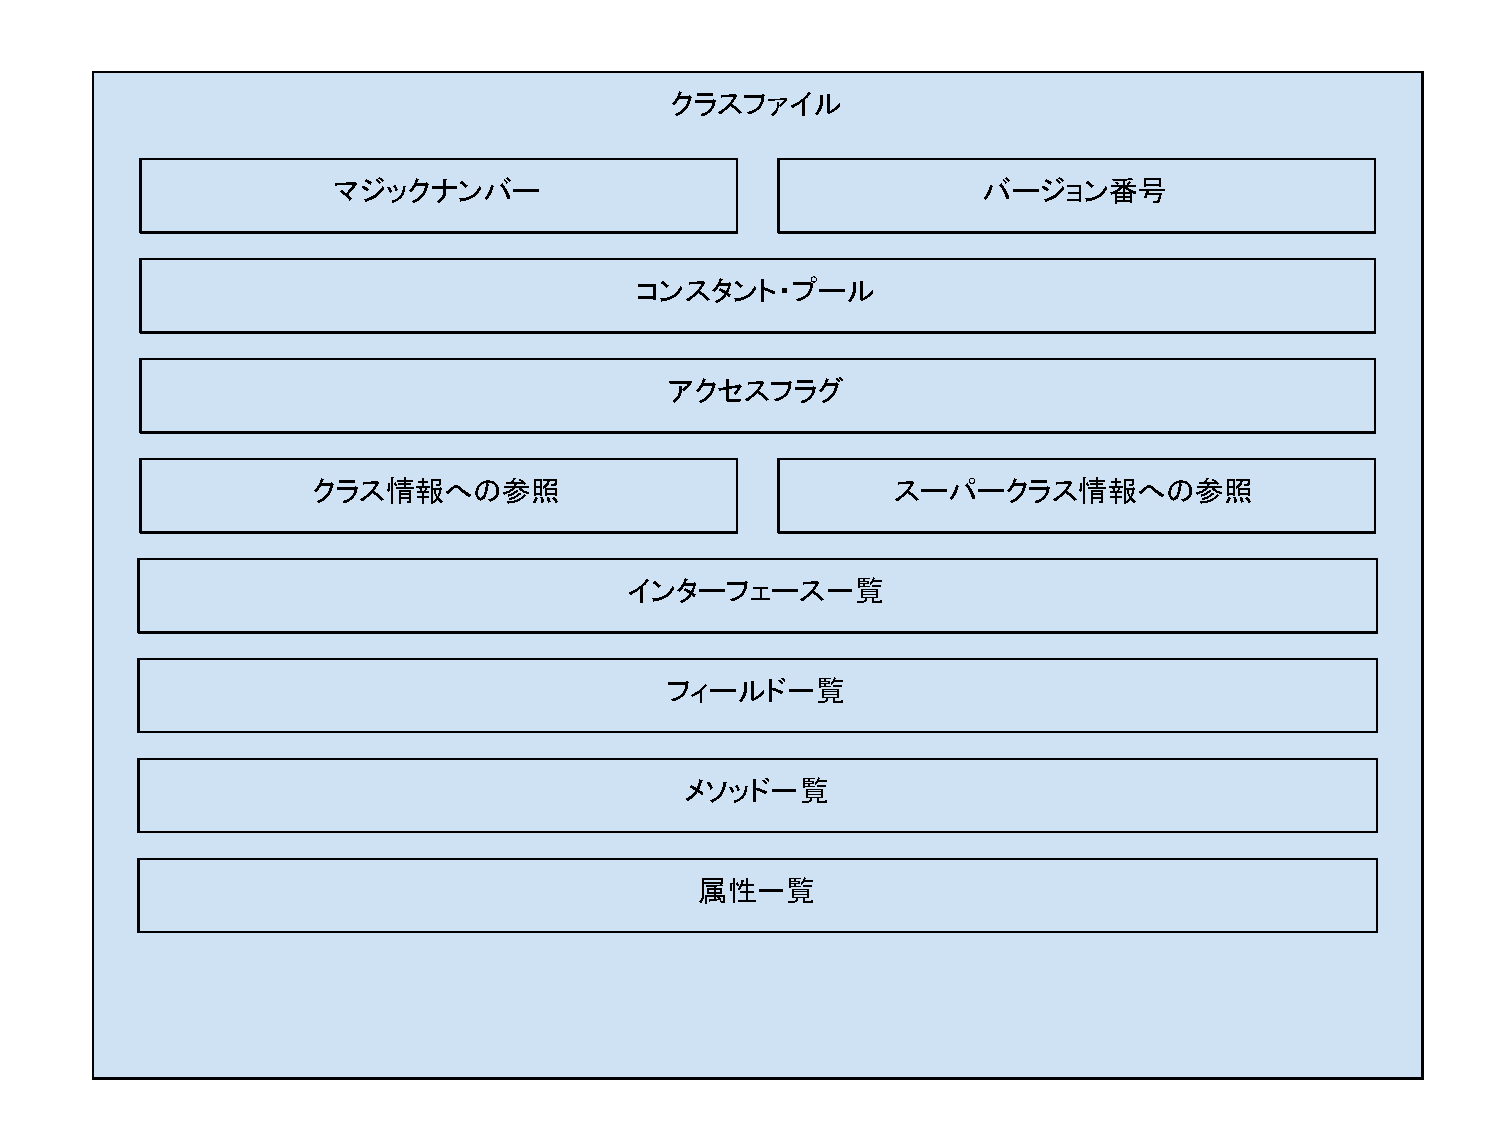
\includegraphics[bb=0 0 800 600,width=12cm]{img/jvm_class_file.pdf}
  \end{center}
\end{figure}

\verb|class|ファイルは、マジックナンバー(\verb|0xCAFEBABE|)と、\verb|class|ファイルのフォーマットのバージョンを表す計4バイトの番号情報を持つ。

コンスタント・プールには、この\verb|class|ファイル内で参照される静的な文字列、クラス名、インターフェース名、フィールド名、メソッド名等の定数が格納されている。

アクセスフラグは、この\verb|class|ファイルがクラスまたはインターフェースのどちらを定義したものか、定義されたクラスまたはインターフェースが外部からアクセス可能か、といった属性を表す。

\verb|class|ファイルは、その\verb|class|ファイルによって定義されるクラスまたはインターフェースを表す情報を指し示すコンスタント・プールへの参照を持つ。

\subsection{構成}

\verb|class|ファイルは、JVMのクラスローダによって読み込まれ、実行される。JVMの構成について、概観を\ref{fig:jvm_architecture}に示す。

\begin{figure}[htbp]
  \caption{JVM構成概観}
  \label{fig:jvm_architecture}
  \begin{center}
    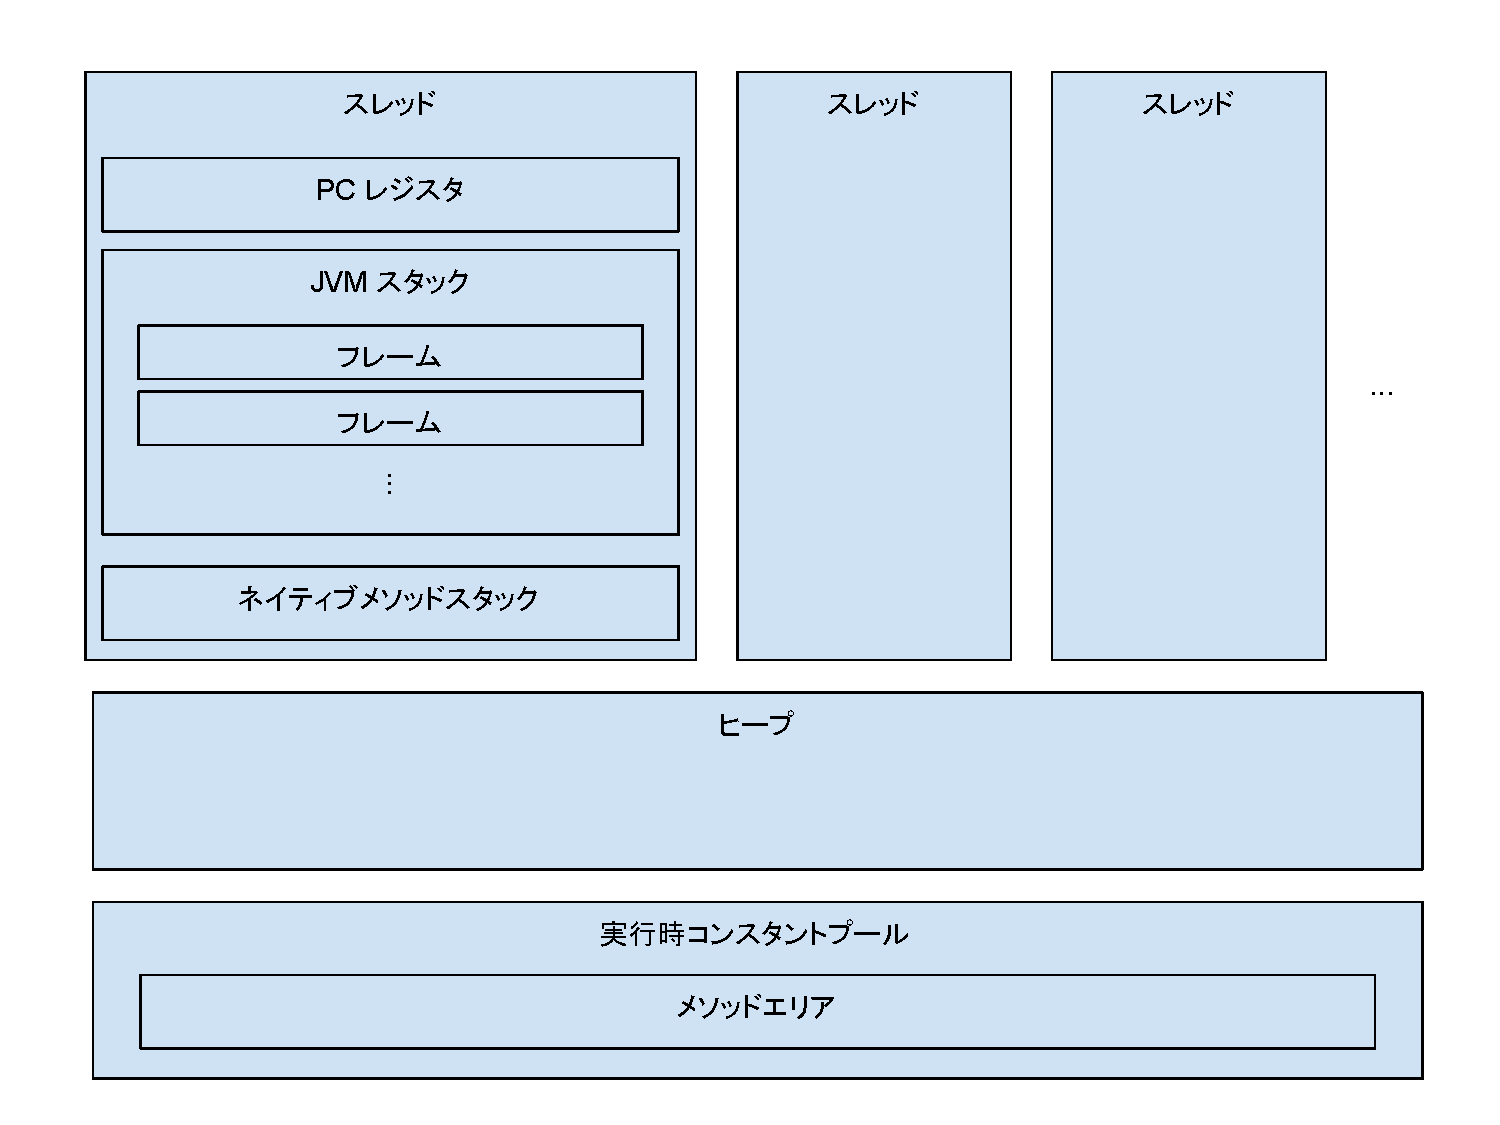
\includegraphics[bb=0 0 800 600,width=12cm]{img/jvm_architecture.pdf}
  \end{center}
\end{figure}

JVMのフレームについて、概観を\ref{fig:jvm_frame}に示す。

\begin{figure}[htbp]
  \caption{JVM構成概観}
  \label{fig:jvm_frame}
  \begin{center}
    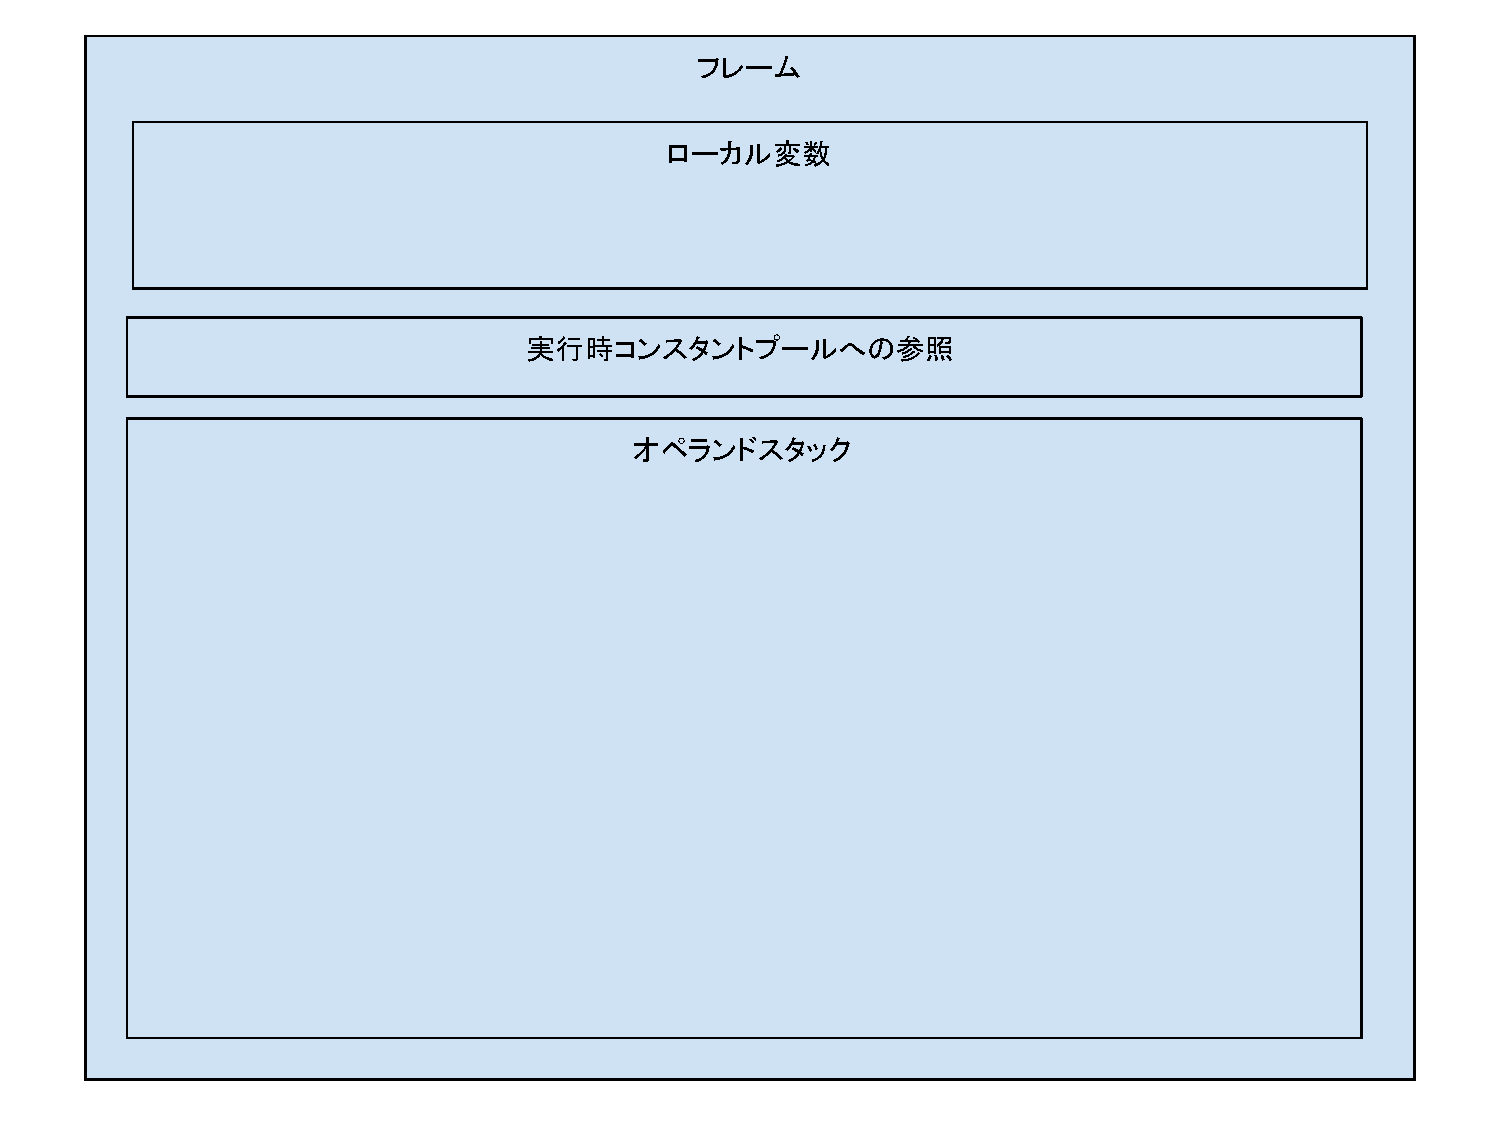
\includegraphics[bb=0 0 800 600,width=12cm]{img/jvm_frame.pdf}
  \end{center}
\end{figure}

\subsection{型}

JVMがサポートする型には、プリミティブ型と\verb|reference|型(参照型)の2種類がある。

プリミティブ型には、数値型と\verb|boolean|型、\verb|returnAddress|型が存在する。

数値型には、以下の7種類が存在する。なお、符号付きの整数は2の補数として表現され、浮動小数点数はIEEE754規格\cite{ieee754}で定められた数値と対応している。
\begin{itemize}
  \item 整数型
  \begin{itemize}
    \item \verb|byte| 符号付き8ビット整数
    \item \verb|short| 符号付き16ビット整数
    \item \verb|int| 符号付き32ビット整数
    \item \verb|long| 符号付き64ビット整数
    \item \verb|char| 符号なし16ビット整数
  \end{itemize}
  \item 浮動小数点数型
  \begin{itemize}
    \item \verb|float| 単精度32ビット形式
    \item \verb|double| 倍精度64ビット形式
  \end{itemize}
\end{itemize}

\verb|boolean|型は、値\verb|true|と\verb|false|をそれぞれ1と0で表したものである。
JVMは\verb|boolean|型の値に対する演算を直接はサポートしておらず、\verb|int|型に変換することで行われる。

\verb|returnAddress|型は、特定の命令へのポインタが値となり、ジャンプ先やリターン先を指定するために用いられる。

\verb|reference|型は、クラス型、インターフェース型、配列型の3種類がある。

\subsection{命令セット}

JVMの命令セットは205の命令を持つ。これらの命令について機能ごとに大別した上で、それぞれの数を表\ref{tb:jvm_opcodes}に示す。

\begin{table}[htbp]
  \caption{JVMが持つ命令セットの分類}
  \label{tb:jvm_opcodes}
  \begin{center}
    \begin{tabular}{|r|r|}
      \hline
      スタックに定数をポップする & 20 \\ \hline
      スタックの操作(値の破棄、複製、スワップ) & 9 \\ \hline
      ローカル変数に対するロード/ストア & 50 \\ \hline
      オブジェクトや配列に対する操作、メソッドの呼び出し & 32 \\ \hline
      型の変換 & 15 \\ \hline
      数値演算 & 37 \\ \hline
      比較 & 21 \\ \hline
      制御(\verb|nop|、\verb|goto|、\verb|return|など) & 14 \\ \hline
      同期処理(\verb|monitor|) & 2 \\ \hline
      例外 & 1 \\ \hline
      その他 & 4 \\ \hline
      \hline
      計 & 205 \\ \hline
    \end{tabular}
  \end{center}
\end{table}

なお、「その他」には、インデックスを2バイトで指定した上で特定の命令を実行する\verb|wide|、
デバッグ用の\verb|breakpoint|、\verb|impdep1|および\verb|impdep2|が含まれる。

\section{WebAssembly}

WebAssemblyは、Google、Microsoft、MozillaおよびAppleの主導によって開発された仮想命令セットである\cite{webassembly}。
従来、WebブラウザにおいてはECMAScriptが事実上唯一の標準化された実行形式であった。
しかし、ECMAScriptはスクリプト言語({\it scripting language})として設計された言語であり\cite{ecma2018}、実行速度や実行効率といった面で最適化されていない。
そこで、WebAssemblyはWebブラウザにおいて高速で安全な実行が可能な形式として設計された。

以下に、WebAssembly実行形式および実行環境の仕様について示す。

\subsection{実行形式}

WebAssemblyでは、プログラムは1つ以上のモジュールに分割される。
WebAssemblyにおけるモジュールの構成を表\ref{fig:wasm_module}に示す。

\begin{figure}[htbp]
  \caption{WebAssemblyモジュール}
  \label{fig:wasm_module}
  \begin{center}
    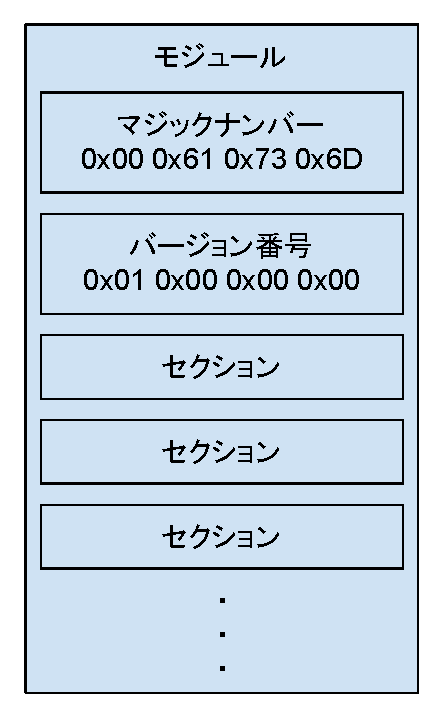
\includegraphics[bb=0 0 800 600,width=12cm]{img/wasm_module.pdf}
  \end{center}
\end{figure}

\subsection{命令セット}

次に、WebAssemblyが持つ命令セットの分類を表\ref{tb:wasm_opcodes}に示す。

\begin{table}[htbp]
  \caption{WebAssemblyが持つ命令セットの分類}
  \label{tb:wasm_opcodes}
  \begin{center}
    \begin{tabular}{|r|r|}
      \hline
      スタックに定数をポップする & 4 \\ \hline
      スタックの操作 & 2 \\ \hline
      ローカル変数に対するロード/ストア & 5 \\ \hline
      メモリ領域に対する操作 & 25 \\ \hline
      型の変換 & 25 \\ \hline
      数値演算 & 64 \\ \hline
      比較 & 34 \\ \hline
      制御(\verb|nop|、\verb|block|、\verb|return|など) & 13 \\ \hline
      \hline
      計 & 172 \\ \hline
    \end{tabular}
  \end{center}
\end{table}
